\documentclass[11pt, a4paper]{article}
\usepackage{amsmath, amsfonts, dsfont, booktabs, graphicx, natbib, a4wide, times, microtype, hyperref}
\newcommand{\E}{\ensuremath{{\mathbb E}}} % expected value
\def\func#1{\mathop{\rm #1}}
\begin{document}
\title{Solution to Exercise 2}
\author{Simon A.\ Broda}
\date{}
\maketitle

\begin{enumerate}
\item
\begin{enumerate}
\item The first thing to observe is the difference between the population quantities (parameters) $\mu$ and $\sigma$, and their estimates $\bar y$ and $s_y$, which are sample quantities. The latter will generally be close to the former because of the law of large numbers, but not the same. The estimates also change every time new random numbers are drawn. The time series plot shows that the observations are randomly scattered around 0. The autocorrelations in the correlogram will mostly be insignificant, i.e., statistically indistinguishable from zero. Formally, the hypothesis being tested is $H_0: \tau_s=0$ vs.\ $H_a: \tau_s\neq0$. Even if $H_0$ is true here, there is still a 5\% probability that any given autocorrelation will be significant; this is called the type-1 error: the probability of rejecting the null even though it is true. A similar statement concerns the $Q$-statistics, which test whether the first $m$ autocorrelations are all equal to zero\footnote{Formally, $Q(m)$ can be used to test $H_0: \tau_1=\tau_2=\ldots=\tau_m=0$.}. \textbf{Important}: make sure to look at the formulas behind the cells and make sure you understand how they work; specifically, the correlogram, the $Q$-stats, and their respective critical values. You don't need to understand how the random numbers $u_t$ themselves are generated (they use a trick called \href{https://en.wikipedia.org/wiki/Inverse_transform_sampling}{inverse transform sampling}).
\item The time series plot looks very different from that in the other sheet, because a random walk is not mean reverting. Also, the correlogram and the $Q$-stats are now highly significant, so that we (correctly) reject the null that the data were generated from a white noise process. In fact, the slow and almost linear decay of the correlogram suggests (correctly) that the data were generated by an integrated process. \textbf{Important}: make sure you understand how the simulated random walk $y_t$ is constructed, by always taking ``yesterday's'' value $y_{t-1}$ and adding $u_t$ to it.
\end{enumerate}
\item
\begin{enumerate}
\item The command \texttt{genr logsp500 = log(sp500)} generates the log prices. From these, the returns can be obtained using the command \texttt{genr r = d(logsp500)}; the \texttt{d} stands for the first difference $\Delta$. Alternatively, the returns can be obtained from the prices directly using the command \texttt{genr r = dlog(sp500)}. The time series plots can be generated like in the exercises for Week 1, resulting in the plots shown in the slides. It is immediately evident that the plot for the returns is very different from that of the (log) prices. This is because the (log) prices are integrated, while returns are stationary. The histogram is obtained by double-clicking the return series, and then clicking \texttt{View$\rightarrow$Descriptive Statistics and Tests$\rightarrow$Histogram and Stats}. This results in the plot below.
\begin{center}
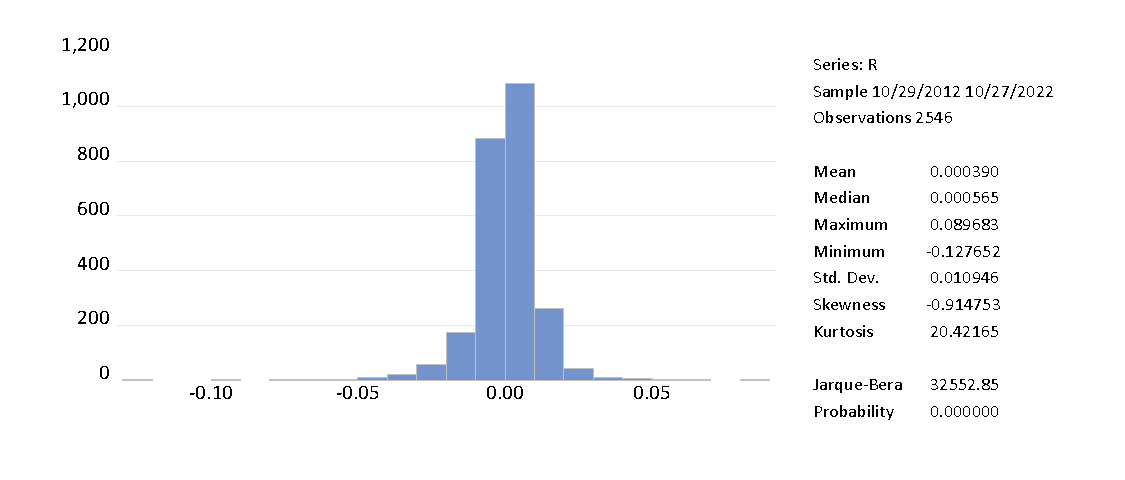
\includegraphics[width=.8\textwidth]{hist_eviews}
\end{center}
\item The output shows a skewness of $\text{SK}=-0.914753$, and a kurtosis of $\text{K}=20.42165$, whereas for a normal distribution, one would expect these values to be close to 0 and 3. This shows that the returns are left-skewed and have heavy tails, a very common finding. Inserting these values, together with $T=2,546$, into the formula
    \[ \text{JB} = \frac{T}{6}\widehat{\text{SK}}^{2} +
   \frac{T}{24}(\widehat{\text{K}}-3)^{2} \]
yields a Jarque-Bera statistic of $\text{JB}=32,552.84$ (up to rounding error, this value is of course already given in the output). This value is much larger than the 5\% critical value of the $\chi^2_2$ distribution, 5.991, so we strongly reject the null that the data were drawn from a normal distribution. We could also have concluded this directly from the $p$-value given in the output, but that might not be available in an exam\ldots
\item The correlogram is obtained by double-clicking the return series, and then clicking \texttt{View$\rightarrow$Correlogram\ldots}. The window that appears allows you to choose the number of lags. Arbitrarily choosing 20 produces the plot below.
\begin{center}
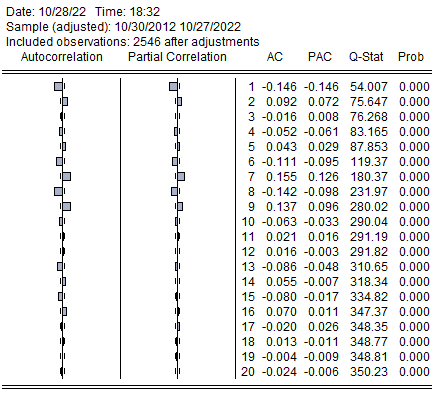
\includegraphics[width=.6\textwidth]{correlogram}
\end{center}
The correlogram doesn't show any indication of non-stationarity, so the data are likely stationary. They don't appear to have been generated by a pure white noise process though, because the autocorrelations and lags 1, 2, 5--10, and 13--17 are significant at the 5\% level; their absolute values exceed the little line representing the critical value $1.96/\sqrt{2546}=0.0388$.
\item The test statistic for testing $H_0: \tau_1=\cdots=\tau_{10}=0$, vs.\ the alternative that at least one of them is non-zero, is
\[
Q(10)=T(T+2)\sum_{s =1}^{10}\frac{\hat{\tau}_{s }^{2}}{T-s }=290.04\sim\chi^2_{10}.
\]
The observed value is 290.04, much larger than the critical value 18.307. Thus, we reject the null and conclude that at least one of the first 10 autocorrelations is different from zero.
\item The correlogram of \texttt{logsp500} looks as follows.
\begin{center}
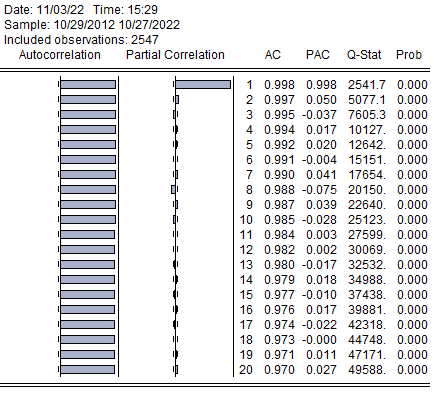
\includegraphics[width=.6\textwidth]{correlogram2}
\end{center}
The autocorrelations are very high, and appear to decay linearly, not exponentially. This is a clear sign the process that generated the data is integrated. It is not a pure random walk though; for a random walk, we would expect that the sample PACF on the right becomes insignificant after the first lag; here, some partial autocorrelations are significant. This, of course, corresponds to the fact that the returns are not pure white noise, as we determined earlier.
\end{enumerate}
\item
\begin{enumerate}
\item By repeatedly plugging in,
\begin{eqnarray*}
Y_t&=&Y_{t-1}+U_t\\
   &=&Y_{t-2}+U_{t-1}+U_t\\
   &=&Y_{t-3}+U_{t-2}+U_{t-1}+U_t\\
&\vdots&\\
&=&Y_0+\sum_{s=1}^t U_s
\end{eqnarray*}
as claimed.
\item The result from the previous question implies that
\begin{align*}
\E\left[Y_t\right]&=\E\left[Y_0+\sum_{s=1}^t U_s\right]\\
&=Y_0+\sum_{s=1}^t \E[U_s]=Y_0.
\end{align*}
Here, we have used that the expectation of a sum is the sum of the expectations, together with the fact that $Y_0$ is assumed to be a constant, and that $\E[U_t]=0$ because $U_t$ is white noise.
For the variance, recall that in general, $\func{var}(X+Y)=\func{var}(X)+\func{var}(Y)+2\func{cov}(X, Y)$. But since the $U_t$ are all independent, we have that $\func{var}(U_s+U_t)=\func{var}(U_s)+\func{var}(U_t)+0=2\sigma^2$. Thus
\begin{align*}
\func{var}\left[Y_t\right]&=\func{var}\left[Y_0+\sum_{s=1}^t U_s\right]\\
&=\func{var}\left[\sum_{s=1}^t U_s\right]\\
&=\sum_{s=1}^t \func{var}(U_s)\\
&=\sum_{s=1}^t \sigma^2\\
&=t\cdot\sigma^2.
\end{align*}

\end{enumerate}

\end{enumerate}
\end{document} 